\chapter{Evaluation}

% Least Squares Linear Regression
% p73 onwards https://people.cs.uchicago.edu/~mrocklin/storage/dissertation.pdf

\begin{guidance}
    For any practical projects, you should almost certainly have
    some kind of evaluation, and it's often useful to separate
    this out into its own chapter.
\end{guidance}

\prechapter{%
    I will evaluate the central premise of this thesis: linear types are a
    practical and usable tool to help working programmers write readable, safe
    (with respect to aliasing, read/write permissions, memory re-use and
    deallocation) and explicit (with respect to memory allocation) code that
    (1) is more memory-efficient than code written using high-level
    linear algebra libraries and (2) performs just as predictably as code
    written using low-level linear-algebra libraries. I will also elaborate on
    the qualitative benefits of using linear types to write linear-algebra
    programs.
}%

\section{Set-up}

I analysed four implementations of a Kalman filter, increasing
the abstraction level at each step:

\begin{enumerate}

    \item a CBLAS/LAPACKE implementation, handwritten in C
        (Figure~\ref{fig:cblas_kalman}), with a minimal number of temporaries,
        calls to `symm' for matrices known to be symmetric ahead of time,
        transposition passed in to `gemm' as a flag and Cholesky decomposition
        for multiplying by an inverse of a matrix

    \item a LT4LA implementation (Figure~\ref{fig:ltfla_kalman}), also with a
        minimal number of temporaries, calls to `symm' for matrices known to be
        symmetric ahead of time, transposition passed in to `gemm' as a flag
        and Cholesky decomposition for multiplying by an inverse of a matrix

    \item an Owl/OCaml implementation using a Cholesky decomposition
        (Figure~\ref{fig:chol_owl_kalman}) but not taking advantage of matrices
        known to be symmetric ahead of time, and producing a new temporary
        matrix for every operation (including inverse and transpose)

    \item an idiomatic Owl/OCaml implementation
        (Figure~\ref{fig:chol_owl_kalman}) with an explicit inverse (LU
        decomposition), not taking advantage of matrices known to be symmetric
        ahead of time, and producing a new temporary matrix for every operation
        (including inverse and transpose).

\end{enumerate}

\begin{sidewaysfigure}

    \begin{minted}[linenos, fontsize=\small]{c}
static void kalman(
    const int n,               const int k,                const double *sigma, /* n,n */
    const double *h, /* k,n */ const double *mu, /* n,1 */ double *r,           /* k,k */
    double *data,    /* k,1 */ double **ret_mu,  /* k,1 */ double **ret_sigma   /* n,n */
) {
        double* k_by_n = (double *) malloc(k * n * sizeof(double));
/*20*/  cblas_dsymm(CblasRowMajor, CblasRight, CblasUpper, k, n, 1., sigma, n, h, n, 0., k_by_n, n);
/*21*/  cblas_dgemm(CblasRowMajor, CblasNoTrans, CblasTrans, k, k, n, 1., k_by_n, n, h, n, 1., r, k);
/*22*/  cblas_dgemm(CblasRowMajor, CblasNoTrans, CblasNoTrans, k, 1, n, 1., h, n, mu, 1, -1., data, 1);
/*23*/  cblas_dcopy(k * n, h, 1, k_by_n, 1);
        double* k_by_k = (double *) malloc(k * k * sizeof(double));
/*24*/  cblas_dcopy(k * k, r, 1, k_by_k, 1);
/*25*/  LAPACKE_dposv(LAPACK_ROW_MAJOR, 'U', k, n, k_by_k, k, k_by_n, n);
/*27*/  LAPACKE_dpotrs(LAPACK_ROW_MAJOR, 'U', k, 1, k_by_k, k, data, 1);
        free(k_by_k);
        double* n_by_n = (double *) malloc(n * n * sizeof(double));
/*28*/  cblas_dgemm(CblasRowMajor, CblasTrans, CblasNoTrans, n, n, k, 1., h, n, k_by_n, n, 0., n_by_n, n);
        free(k_by_n);
        double* n_by_1 = (double *) malloc(n * sizeof(double));
/*29*/  cblas_dgemm(CblasRowMajor, CblasTrans, CblasNoTrans, n, 1, k, 1., h, n, data, 1, 0., n_by_1, 1);
        double* new_mu = (double *) malloc(n * sizeof(double));
/*30*/  cblas_dcopy(n, mu, 1, new_mu, 1);
/*31*/  cblas_dsymm(CblasRowMajor, CblasLeft, CblasUpper, n, 1, 1., sigma, n, n_by_1, 1, 1., new_mu, 1);
        free(n_by_1);
        double* n_by_n2 = (double *) malloc(n * n * sizeof(double));
/*32*/  cblas_dsymm(CblasRowMajor, CblasRight, CblasUpper, n, n, 1., sigma, n, n_by_n, n, 0., n_by_n2, n);
/*33*/  cblas_dcopy(n*n, sigma, 1, n_by_n, 1);
/*34*/  cblas_dsymm(CblasRowMajor, CblasLeft, CblasUpper, n, n, -1., sigma, n, n_by_n2, n, 1., n_by_n, n);
        free(n_by_n2);
        *ret_sigma = n_by_n;
        *ret_mu = new_mu;
}
    \end{minted}
    \caption{CBLAS/LAPACKE implementation of a Kalman filter. I used C instead
        of Fortran because it is what Owl uses under the hood and OCaml FFI
        support for C is better and easier to use than that for Fortran. A distinct
        `measure\_kalman' function that sandwiches a call to this function with
        \texttt{getrusage} is omitted for brevity.}\label{fig:cblas_kalman}

\end{sidewaysfigure}

\begin{figure}[tp]
    \begin{minted}[linenos, fontsize=\small]{ocaml}
let potrs ~uplo a b =
  let b = Owl.Mat.copy b in
  Owl.Lapacke.potrs ~uplo ~a ~b
;;

let chol_kalman ~sigma ~h ~mu ~r ~data =
  let open Owl.Mat in
  let ( * ) = dot in
  let h' = transpose h in
  let sigma_h' = sigma * h' in
  let chol = Owl.Linalg.D.chol (r + h * sigma_h') in
  let sigma_h'_inv rest = sigma_h' * potrs ~uplo:'U' chol rest in
  let new_sigma = sigma - sigma_h'_inv (h * sigma) in
  let new_mu = mu + sigma_h'_inv (h * mu - data) in
  ((sigma, (h, (mu, (r, data)))), (new_mu, new_sigma))
;;

let owl_kalman ~sigma ~h ~mu ~r ~data =
  let open Owl.Mat in
  let ( * ) = dot in
  let h' = transpose h in
  let sigma_h' = sigma * h' in
  let x = sigma_h' * (inv @@ r + h * sigma_h') in
  let new_mu = mu + x * (h * mu - data) in
  let new_sigma = sigma - x * h * sigma in
  ((sigma, (h, (mu, (r, data)))), (new_mu, new_sigma))
;;
    \end{minted}
    \caption{Implementations of a Kalman filter using Owl, top one using a
        Cholesky decomposition, bottom one using idiomatic Owl. Owl does not
        yet provide a non-mutating `potrs' function, so I wrote my own which
        returns a mutated copy of its argument instead.}\label{fig:chol_owl_kalman}

\end{figure}

I evaluated the implementations on two metrics: memory usage (via number and
size of temporaries allocated) and execution time. For the former, I compiled
Owl with print-statements on the relevant primitives to see exactly the number
of temporaries allocated for a single call of each function. While I did also
attempt to use gperftools and OCaml's profiling support with gprof for a more
holistic view of memory usage in the presence of OCaml's garbage-collector, I
ran into technical difficulties irrelevant to this thesis.

I measured execution time, in micro-seconds, against an exponentially (powers
of 5) increasing scaling factor for matrix size parameters $n=5$ and $k=3$.
For small scaling factors (1, 5, 25), I used the Core\_bench micro-benchmarking
library, for larger factors (125 and greater), I used the \texttt{getrusage}
system call (called \ltfla{Unix.times} in OCaml), sandwiched between calls to
\ltfla{Gc.full_major} to ensure no garbage collection took place during the
measurements.  Core\_bench performs a linear-regression (here, time against
batch-size) so includes 95\% confidence-interval with $R^2$. Larger scales have
errors reported to $\pm \sigma$ (one standard-deviation) 

\section{Results}

All implementations produce the same answers (within at most $2^{-52}$). Raw
output of implementation traces and the benchmarking program (including sample
sizes) for each of the implementations are in Appendix~\ref{chap:eval_data}.

\subsection{Memory Usage}

Inspecting the Owl trace shows generated 11 temporary matrices (13 calls to
empty, 2 of which are the resulting matrices). Chol shows 13 temporaries (same
as Chol plus two temporaries for the two calls to potrs), whereas both LT4LA
and CBLAS have 4 temporaries. Analysing the sub-expressions of the Owl
implementation shows the total amount of memory allocated for temporaries is $n
+ n^2 + 4nk + 3k^2 + 2k$ words; for Chol the total is that of Owl plus $n +
nk$; for LT4LA and CBLAS the total is $n + n^2 + nk + k^2$.

\subsection{Execution Time}

A graph of the execution times (with error bars which are present but quite
small) is show in Figure~\ref{fig:timings}.

\begin{figure}[tp]
    \centering
    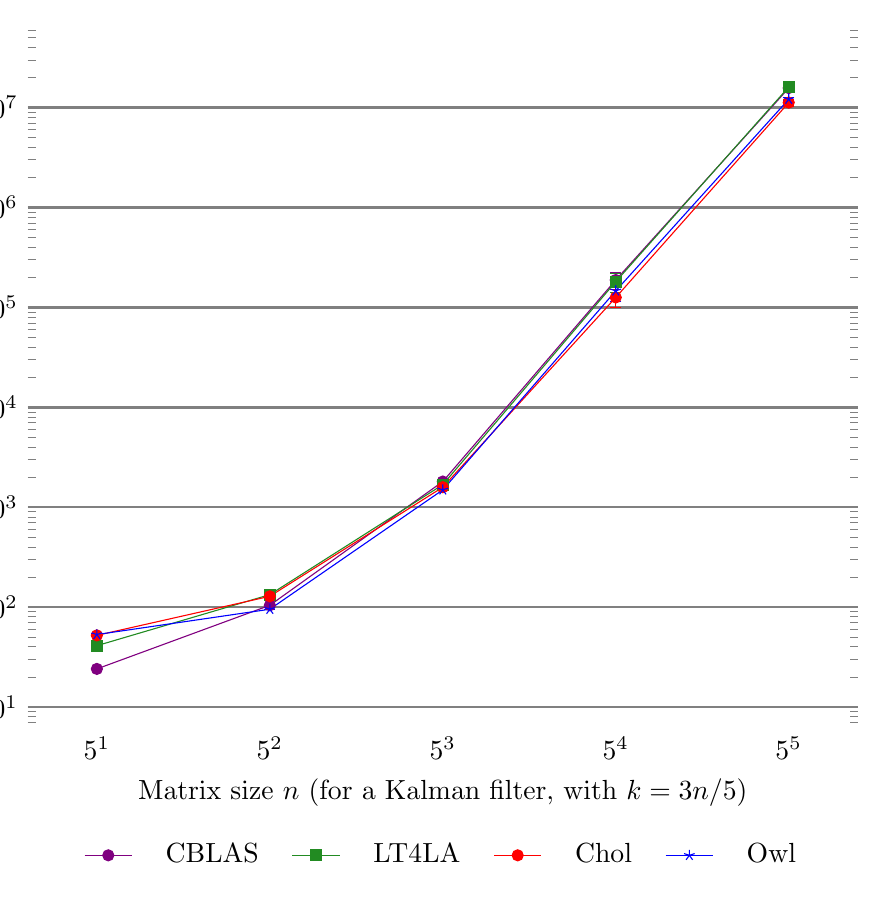
\begin{tikzpicture}[trim axis left]
\begin{axis}[
    % width of chart
    width=\textwidth,
    % no box, below chart, horizontal
    legend style={%
      draw=none,
      at={(0.5,-0.15)},
      anchor=north,
      legend columns=4,
      column sep = 1em,
      cells={align=center},
    },
    % log ticks with fixed point,
    % yticklabel={\pgfmathparse{pow(10,\tick-3)}\pgfmathprintnumber[fixed]{\pgfmathresult}}\,ms, % N ms along y-axis
    % xticklabel={\pgfmathparse{pow(5,\tick)}\pgfmathprintnumber[fixed]{\pgfmathresult}},
    xlabel near ticks,
    xlabel={Matrix size $n$ (for a Kalman filter, with $k=3n/5$)},
    ylabel near ticks,
    ylabel={Execution time of one call to Kalman filter ($\mu$s)},
    xmode = log,
    log basis x = {5},
    axis line style={opacity=0}, % hide y axis
    major tick style={draw=none}, % no ticks
    ymode=log, % log scale for y
    log basis y = {10}, % log base 10
    ymajorgrids, % rows of lines
    major grid style={gray, line width=1pt},
]

  % CBLAS
    \addplot+ [
        violet,
        mark options={fill=violet},
        error bars/.cd, y dir=both, y explicit,
    ] table [
        y error plus=ey+,
        y error minus=ey-,
    ] {
         x         y     ey+     ey-
         5        24       0       0
        25       104       1       1
       125      1803      64      57
       625    187667   36281   36281
      3125  15651064  530675  530675
  };

  % LT4LA
    \addplot+ [
        ForestGreen,
        mark options={fill=ForestGreen},
        error bars/.cd, y dir=both, y explicit,
    ] table [
        y error plus=ey+,
        y error minus=ey-,
    ] {
         x         y     ey+     ey-
         5        41       1       1
        25       133       2       2
       125      1678      36      33
       625    180575   38386   38386
      3125  16061291  193746  193746
  };

  % Chol
    \addplot+ [
        red,
        mark options={fill=red},
        error bars/.cd, y dir=both, y explicit,
    ] table [
        y error plus=ey+,
        y error minus=ey-,
    ] {
         x         y     ey+     ey-
         5        52       1       1
        25       128       1       1
       125      1583      95      75
       625    125526   25502   25502
      3125  11210982 852463   852463
  };

  % Owl
    \addplot+ [
        Blue,
        mark options={fill=Blue},
        error bars/.cd, y dir=both, y explicit,
    ] table [
        y error plus=ey+,
        y error minus=ey-,
    ] {
         x         y     ey+      ey-
         5        53       1        1
        25        95       0        0
       125      1488      27       24
       625    146150   32346    32346
      3125  12108640  466381   466381
  };



  \legend{CBLAS,LT4LA,Chol,Owl}

\end{axis}
\end{tikzpicture}

    \caption{Comparison of execution times. Small matrices and timings $n \le
        5^3$ were micro-benchmarked with the Core\_bench library. Larger ones used
        Unix's \texttt{getrusage} functionality, sandwiched between calls to
        \ltfla{Gc.full_major} for the OCaml implementations.}\label{fig:timings}

\end{figure}

For $n=5$, and a per implementation sample size of around 450, the CBLAS
implementation is the fastest ($24\mu s$), followed by LT4LA ($41 \mu s$), then
Cholesky and Owl (around $52 \mu s$).  However, for $n=25$, and around 350
measurements per implementation, the idiomatic Owl implementation is the fastest
($95 \mu s$), \emph{then} CBLAS ($104 \mu s$), with LT4LA and Chol last (around
$130 \mu s$). The 95\% confidence-intervals around these measurements are
between 0 and 2.

For $n=125$, and a per implementation sample size of around 110, the trends change:
CBLAS implementation is now the \emph{slowest} ($1803 \mu s\, [1746,\, 1867]$).
This is followed by LT4LA ($1678 \mu s\, [1646,\, 1714]$) and Owl ($1488 \mu
s\, [1464,\, 1515]$). Chol had a low $R^2$ value ($0.74$) and so its execution
time is inconclusive here.

For $n=625$ and a sample size of 1000, Chol was now the fastest ($125.5 \pm
25\,ms$), then Owl ($146 \pm 32 \,ms$), followed by LT4LA ($180.5 \pm 38 \,ms$)
and CBLAS ($188 \pm 36 \, ms$). Despite the large sample size, the
standard-deviation is still quite high; however, \emph{because} of the large
sample size, the pair-wise $p$-values (Welch's t-test) are very small ($p <
.05$), suggesting that the difference in the means is statistically
significant.

For $n=3125$ and a sample size of 15, Chol and Owl had similar mean execution
times ($11.2 \pm 0.85 \,s$ and $12.1 \pm 0.47 \,s$ respectively) while LT4LA
and CBLAS had similar, but \emph{slower} mean execution times ($16.1 \pm 0.19
\,s$ and $15.7 \pm 0.53 \,s$ respectively). Pair-wise $p$-values (Welch's
t-test) are all less than $.05$, so the differences in means are statistically
significant.

\section{Analysis}

Having access to primitives which allow a programmer to re-use memory means
that memory usage for temporaries in LT4LA is on par with that of CBLAS. One
caveat is that the \ltfla{freeM} primitive is a no-op in LT4LA, so deallocation
still relies on OCaml's garbage-collector. The difference between these two
implementations and the idiomatic Owl implementation is $k(3n+2k+2)$ words.

For small matrix sizes, LT4LA and CBLAS execution times differ. I suspect this
is due to large sample sizes causing more allocations and thus more
garbage-collector unpredictability (which the linear-regression \emph{did not}
take into account; multi-variate regressions are not fully supported
Core\_bench yet).

As matrix size increases, execution times of LT4LA become very similar to those
of CBLAS. However, that does not necessarily mean faster.  Especially for
$n=625$ and $n=3125$ (sizes for which \ltfla{Gc.full_major} was called before
each measurement), mean execution times start to split clearly into two groups:
Chol and Owl as one group (similar, faster times) and LT4LA and CBLAS as
another (similar, slower times).

Overall, as far as memory usage is concerned, it is possible to write linear
algebra programs with the safety (with respect to aliasing and read/write
permissions) of using high-level libraries whilst gaining the explicit control
over memory allocation and re-use associated with low-level libraries.
As far as execution times are concerned, even though the idiomatic OCaml
implementations seem to be faster for this particular
benchmark,\footnote{Attempting to understand \emph{why} the
    Chol/Owl implementations tended to be faster for anything except the
    smallest of matrices, despite allocating almost twice the number of
    temporaries was difficult. Running the different implementations through
    the Cachegrind cache simulator (part of Valgrind) showed that LT4LA/CBLAS
    had a roughly 1\% higher cache miss rate than Chol/Owl (rising from around
    11\% to around 12\%). This seemed insufficient to account for the
    differences, so I investigated further. I added an extra, modified
    implementation of LT4LA, which transposed the `h' parameter into a new
    matrix rather than using the transpose flag to `gemm', to see if
    row-vs-column access patterns could account for the differences (they did
    not). Had I been able to use gprof or gperftools, I would have profiled the
    remaining key difference: the `symm' routine (which performs \emph{half} as
    many multiplications as `gemm' because it knows one of its
    arguments is symmetric).}
we can conclude that LT4LA performs similarly to using lower-level libraries
when garbage-collection is controlled for and especially as matrix sizes increase.

\section{Limitations}

I chose the example of a Kalman filter because it is used in the real world,
consists purely of a sequence of matrix expressions and produces many
unnecessary temporary matrices when implemented idiomatically in a high-level
linear-algebra library. It is good for isolating the key differences between
not having and having linear types to help a programmer safely manage memory
and aliasing, whilst excluding other aspects also important to real world
linear-algebra programs such as control flow or blocking.

\section{Qualitative Benefits}

Prior to this project, I had no experience with linear-algebra libraries or the
problem of matrix expression compilation. As such, I based my initial LT4LA
implementation of a Kalman filter using BLAS and LAPACK, on a popular GitHub
gist of a Fortran implementation, one that was automatically generated from
SymPy's matrix expression compiler~\cite{rocklin_thesis}.

Once I translated the implementation, I attempted to compile it and found that
(to my surprise) it did not type-check. This was because the original
implementation contained incorrect aliasing, did not adhere to Fortran's
read/write permissions (with respect to \texttt{intent} annotations
\texttt{in}, \texttt{out} and \texttt{inout}) and unused and unnecessary
temporaries, all of which were now highlighted by LT4LA's type system.

The original implementation used 6 temporaries, one of which was immediately
spotted as not being used due to linearity. It also contained two variables
which were marked as \texttt{intent(in)} but would have been written over by
calls to `gemm', spotted by the fractional-capabilities feature. Furthermore,
it used a matrix \emph{twice} in a call to `symm', once with a read permission
but once with a \emph{write} permission.  Fortran assumes that any parameter
being written to is not aliased and so this call was not only incorrect, but
illegal according to the standard, both aspects of which were captured by
linearity and fractional-capabilities. Lastly, it contained another unnecessary
temporary, however one that was not obvious without linear types. To spot it, I
first performed live-range splitting (checked by linearity) by hoisting calls
to \ltfla{freeM} and then annotated the freed matrices with their dimensions.
After doing so and spotting two disjoint live-ranges of the same size, I
replaced a call to \ltfla{freeM} followed by allocating call to \ltfla{copy}
with one, in-place call to \ltfla{copyM_to}.


\section{Summary}

Writing a linear-algebra program using LT4LA gives a programmer both
\emph{explicit control} (over read/write permissions, aliasing and memory
allocation, re-use and deallocation) and \emph{signals intent} to the compiler
and reader clearly without sacrificing either of readability or
value-semantics. The resulting programs perform similarly to equivalent
programs written directly using lower-level linear-algebra libraries. In turn,
the programs written can be \emph{checked automatically} against their intent,
especially when \emph{refactoring} or \emph{rewriting} code. Although any
expert \emph{could} have followed the same line of reasoning laid out above,
and arrived at the same program, LT4LA's type system enables a non-expert
(yours truly) to do the same and increase confidence in the result\footnote{As
always, this does not preclude testing code by actually executing it, but
definitely \emph{complements} it.} by checking said line of reasoning.
